\documentclass[conference]{IEEEtran}
\IEEEoverridecommandlockouts
\IEEEpubid{\makebox[\columnwidth]{XXX-X-XXXX-XXXX-X/XX/\$XX.00~\copyright 20XX IEEE\hfill}\hspace{\columnsep}\makebox[\columnwidth]{}}
% Times, as in the IEEE template (tectonic/XeTeX has no ptm in TU encoding)
\usepackage[T1]{fontenc}
\usepackage{amsmath}
\usepackage{newtxtext,newtxmath}
\usepackage{graphicx}
\usepackage{booktabs}
\usepackage{xcolor}
\usepackage{url}

% Every \tbd{} is a value that has NOT been measured yet. Do not submit while any remain.
\renewcommand{\IEEEkeywordsname}{Keywords}
\newcommand{\tbd}[1]{\textcolor{red}{\textbf{[TBD: #1]}}}

\begin{document}

\title{Handwritten Mathematical Expression Recognition with a Classic Attention-LSTM: Staged Transfer Learning and a Comparison with a Transformer Baseline}

\author{\IEEEauthorblockN{Hardik Khaneja}
\IEEEauthorblockA{\textit{Manipal Institute of Technology}\\
Manipal, India}
\and
\IEEEauthorblockN{Dhruva R.M. Upadhaya}
\IEEEauthorblockA{\textit{Manipal Institute of Technology}\\
Manipal, India}
\and
\IEEEauthorblockN{Rijul Bhatia}
\IEEEauthorblockA{\textit{Manipal Institute of Technology}\\
Manipal, India}}

\maketitle
\IEEEpubidadjcol

\begin{abstract}
We study image-to-\LaTeX{} recognition of mathematical expressions with a deliberately classic encoder--decoder: a ResNet-18 convolutional encoder, additive (Bahdanau) attention and an LSTM decoder with beam search. The model is trained in three stages that move progressively further from clean, printed input: printed formulas (im2latex-100k), handwritten expressions (MathWriting) and photographed handwriting (HME100K). A single 429-token vocabulary is shared by all stages, so each stage warm-starts from the previous one without resizing the output layer. Images are resized with their aspect ratio preserved and attention is masked so that padding is never attended to. On held-out subsets the model reaches a BLEU of 91.5 on printed formulas and 79.4 on handwritten expressions, with expression-level exact match (ExpRate) of 0.47 and 0.32 respectively. We compare against pix2tex, an open-source vision-transformer model, under an identical tokenizer and metric implementation; used off the shelf, it recognizes none of 500 handwritten test expressions exactly, showing the size of the printed-to-handwritten domain gap \tbd{im2latex/HME100K comparison}, and ablate a finer encoder grid, coverage attention and photo-style augmentation \tbd{one-sentence ablation finding}.
\end{abstract}

\begin{IEEEkeywords}
handwritten mathematical expression recognition, image-to-markup, attention, encoder--decoder, transfer learning
\end{IEEEkeywords}

%=====================================================================
\section{Introduction}
Converting an image of a mathematical expression into \LaTeX{} is harder than ordinary text recognition. Symbols are arranged in two dimensions (fractions, sub- and superscripts, radicals), the output is a long structured token sequence, and handwriting adds large variation in stroke shape, size and spacing. Photographs of handwriting add a further domain gap: perspective, uneven lighting, blur and compression artefacts.

Recent systems for this task use transformer decoders and, increasingly, vision-transformer encoders. Such models are data- and compute-hungry. This paper asks a practical question: \emph{how far does a classic, interpretable CNN--attention--LSTM model go when trained on a limited compute budget, and what does a modern transformer model buy over it?}

Our contributions are:
\begin{itemize}
\item A from-scratch implementation of a ResNet-18 + Bahdanau attention + LSTM image-to-\LaTeX{} model with aspect-preserving preprocessing and pad-masked attention (Section~\ref{sec:method}).
\item A three-stage transfer-learning recipe (printed $\rightarrow$ handwritten $\rightarrow$ photographed) with a single shared vocabulary, and measurements after each stage (Section~\ref{sec:results}).
\item A comparison with pix2tex using one shared tokenizer and metric implementation, so both models are scored identically.
\item An ablation of three design choices: encoder grid resolution, coverage attention and photo-style data augmentation.
\end{itemize}

We frame the study around three research questions:
\begin{description}
\item[RQ1] How does the classic model compare with a transformer-based model (pix2tex) on the same test images?
\item[RQ2] How does accuracy change across the printed, handwritten and photographed stages?
\item[RQ3] How much does each of the finer encoder grid, coverage attention and photo-style augmentation contribute?
\end{description}

%=====================================================================
\section{Related Work}
\textbf{Image-to-markup.} Deng et al.~\cite{deng2017im2markup} framed formula recognition as image-to-markup generation with a convolutional encoder and attention-based recurrent decoder, and released the im2latex-100k dataset of rendered formulas. Zhang et al.~\cite{zhang2017wap} proposed Watch, Attend and Parse (WAP) for handwritten expressions, using a fully convolutional encoder and an attention-based GRU decoder with a coverage vector.

\textbf{Attention.} Additive attention was introduced by Bahdanau et al.~\cite{bahdanau2015} for machine translation. Xu et al.~\cite{xu2015show} applied it to image captioning and introduced a doubly stochastic regularizer that encourages every image region to receive attention over the course of decoding. Tu et al.~\cite{tu2016coverage} introduced coverage, which feeds accumulated past attention back into the attention model to reduce repeated and skipped inputs.

\textbf{Transformer-based recognizers.} pix2tex (LaTeX-OCR)~\cite{pix2tex} is an open-source model that pairs a vision-transformer encoder with a transformer decoder, trained primarily on rendered formulas.

\textbf{Datasets.} MathWriting~\cite{mathwriting} is a large dataset of online handwritten expressions, of which we use the human-written portion in pre-rendered image form. HME100K~\cite{hme100k} consists of photographed handwritten expressions captured in real-world conditions.

%=====================================================================
\section{Methodology}\label{sec:method}

\subsection{Preprocessing}
Each image is converted to grayscale and replicated to three channels so that the ImageNet-pretrained first convolution remains valid. It is then scaled to a fixed height of 128 pixels \emph{preserving its aspect ratio}; only images wider than 1024 pixels after scaling are scaled down further, still without distortion. Images in a batch are right-padded to the widest image, and each sample carries its valid height and width so that the padding can be masked out of attention. Pixel values are normalized with ImageNet statistics.

\subsection{Encoder}
The encoder is a ResNet-18~\cite{he2016resnet} with its average-pool and classification layers removed, followed by a $1{\times}1$ convolution projecting 512 channels to $d_e = 256$. The $H'{\times}W'$ feature map is flattened into a sequence of $H'W'$ annotation vectors $\{\mathbf{e}_i\}$. By default the backbone has total stride 32; the \emph{fine-grid} variant sets the stride of the first block of the last stage to 1, giving total stride 16 (8 feature rows rather than 4 at height 128).

\subsection{Attention}
At decoding step $t$, with decoder hidden state $\mathbf{h}_{t-1}$, attention energies are
\begin{equation}
s_{t,i} = \mathbf{v}^\top \tanh\!\left(W_e\mathbf{e}_i + W_d\mathbf{h}_{t-1} + \mathbf{w}_c\, c_{t,i}\right),
\end{equation}
where $c_{t,i}=\sum_{k<t}\alpha_{k,i}$ is the coverage of cell $i$. The coverage term is present only in the coverage variant; its weights are initialized to zero, so a model warm-started from a checkpoint without coverage initially produces identical outputs. Energies at padded cells are set to a large negative value before the softmax, so $\alpha_{t,i}\approx 0$ on padding. The context vector is $\mathbf{z}_t=\sum_i \alpha_{t,i}\mathbf{e}_i$.

\subsection{Decoder}
An LSTM cell with hidden size 256 takes the concatenation of a 128-dimensional token embedding and $\mathbf{z}_t$. Its initial hidden and cell states are linear projections of the mean of the valid (unpadded) annotation vectors. Output logits are a linear function of $[\mathbf{h}_t;\mathbf{z}_t]$ after dropout (0.3). The attention dimension is 128.

\subsection{Training objective}
The loss is token-level cross-entropy (padding ignored) plus the doubly stochastic attention regularizer of~\cite{xu2015show}:
\begin{equation}
\mathcal{L} = \mathcal{L}_{\mathrm{CE}} + \lambda \cdot \tfrac{1}{N}\sum_i \Bigl(1-\textstyle\sum_t \alpha_{t,i}\Bigr)^2, \qquad \lambda = 1.
\end{equation}
Training uses teacher forcing with ratio starting at 1.0, reduced by 0.02 per epoch to a floor of 0.5.

\subsection{Inference and confidence}
We decode with beam search (width 5, maximum length 200) and rank finished hypotheses by $\log p / L^{0.7}$, where $L$ is the hypothesis length. The reported confidence is the length-normalized probability $\exp(\log p / L)$ of the selected hypothesis.

\subsection{Tokenization}
\LaTeX{} strings are split by a regular-expression tokenizer into commands (e.g.\ \verb|\frac|), single characters and braces. A vocabulary of 429 tokens (including four special tokens: padding, start, end and unknown) is built once from the im2latex-100k training set and reused unchanged for every later stage.

%=====================================================================
\section{Experimental Setup}\label{sec:setup}

\subsection{Datasets}
Table~\ref{tab:data} summarizes the data used at each stage.
\begin{itemize}
\item \textbf{Stage 1 (printed):} im2latex-100k~\cite{deng2017im2markup}, using its train, validation and test splits.
\item \textbf{Stage 2 (handwritten):} the human-written portion of MathWriting~\cite{mathwriting}, capped at 40{,}000 training and 4{,}000 validation images. The synthetic portion is not used. The stage-1 vocabulary covers 99.9\% of MathWriting tokens.
\item \textbf{Stage 3 (photographed):} HME100K~\cite{hme100k}. The public mirror we used provides labels for the training set only, so we split it into training, validation and test portions of approximately 70k, 2k and 2k images. \emph{Our HME100K test set is therefore a held-out slice of the original training distribution, not the official HME100K test set, and our numbers are not comparable with published HME100K results.}
\end{itemize}

\begin{table}[t]
\caption{Data used at each training stage.}
\label{tab:data}
\centering
\begin{tabular}{llrrr}
\toprule
Stage & Dataset & Train & Val & Test \\
\midrule
1 & im2latex-100k & \tbd{n} & \tbd{n} & \tbd{n} \\
2 & MathWriting (human) & 40{,}000 & 4{,}000 & \tbd{n} \\
3 & HME100K (self-split) & $\approx$70k & $\approx$2k & $\approx$2k \\
\bottomrule
\end{tabular}
\end{table}

\subsection{Training}
Stage 1 trains from ImageNet-initialized ResNet-18 weights with Adam (learning rate $10^{-3}$, weight decay $10^{-5}$), batch size 32 and gradient-norm clipping at 5.0. The learning rate is reduced on a validation-loss plateau (patience 2). Stages 2 and 3 warm-start from the previous stage's best checkpoint with learning rate $10^{-4}$. The best checkpoint at each stage is selected by validation cross-entropy. The best checkpoint was reached at epoch 32 in stage 1, epoch 25 in stage 2 and epoch 14 in stage 3 \tbd{total epochs run per stage}. All training was run on Kaggle (\tbd{GPU model}); wall-clock time per stage was \tbd{hours}.

Training-time augmentation (applied on the fly):
random affine transform (rotation and shear up to $5^\circ$, translation up to 2\%), Gaussian blur and brightness/contrast jitter. The \emph{photo-style} augmentation used in the ablation adds random perspective distortion, a linear shadow gradient, stronger blur and jitter, and JPEG re-encoding at quality 20--60.

\subsection{Model variants}
All results in Tables~\ref{tab:stages}--\ref{tab:pix2tex} use the \emph{baseline} configuration: total encoder stride 32, no coverage, and the lighter augmentation above. The ablation (Table~\ref{tab:ablation}) adds the fine grid, coverage and photo-style augmentation one at a time.

\subsection{Metrics}
Predictions and references are tokenized with the same tokenizer and scored by one shared implementation for every model:
\begin{itemize}
\item \textbf{BLEU}: corpus-level 4-gram BLEU~\cite{papineni2002bleu} over tokens (NLTK, smoothing method 4).
\item \textbf{ExpRate}: fraction of expressions whose predicted token sequence matches the reference exactly.
\item \textbf{ExpRate $\le k$}: fraction whose token-level edit distance to the reference is at most $k$, for $k\in\{1,2\}$.
\end{itemize}

%=====================================================================
\section{Results and Analysis}\label{sec:results}

\subsection{RQ2: Accuracy across stages}
Table~\ref{tab:stages} reports each stage's best checkpoint on its own test set. These figures are computed on the first 500 images of each test split, and on the self-split HME100K test slice.

\begin{table}[t]
\caption{Baseline model after each training stage (test subsets of 500 images; HME100K on our self-split held-out slice).}
\label{tab:stages}
\centering
\setlength{\tabcolsep}{4pt}
\begin{tabular}{llrrrr}
\toprule
Stage & Test set & BLEU & ExpRate & $\le$1 & $\le$2 \\
\midrule
1 & im2latex (printed) & 91.5 & 0.470 & 0.550 & 0.700 \\
2 & MathWriting (hand.) & 79.4 & 0.320 & 0.510 & 0.650 \\
3 & HME100K (photos) & 88.3 & 0.524 & 0.724 & 0.832 \\
\bottomrule
\end{tabular}
\end{table}

Moving from printed to handwritten input lowers BLEU from 91.5 to 79.4 and ExpRate from 0.47 to 0.32, reflecting the added difficulty of handwriting. Fine-tuning on MathWriting raised validation token accuracy from 0.52 (the stage-1 model evaluated on MathWriting) to 0.82. Stage-3 validation token accuracy peaked at 0.836. The higher ExpRate on HME100K than on MathWriting should not be read as photographs being easier: the HME100K test slice comes from the same distribution as its training data, and the two test sets differ in expression length and symbol distribution. The 500 MathWriting test expressions average 18.1 tokens (median 17, range 1--72) \tbd{same statistics for the HME100K test slice}.

\textbf{More handwriting data.} Training on the full MathWriting human split for 20 epochs instead of the 40{,}000-image subset (same baseline architecture) raises BLEU on the same 500 test images from 79.4 to 86.7 and ExpRate from 0.316 to 0.478 (ExpRate $\le$1: 0.680, $\le$2: 0.794) \tbd{size of the full training split}.

\textbf{Catastrophic forgetting.} Fine-tuning on photographs degrades handwriting accuracy. On a 200-image slice of the MathWriting test set, the stage-3 (HME100K) checkpoint reaches an ExpRate of only 0.065, whereas a model trained for 20 epochs on the full MathWriting human split reaches 0.445 on the same slice.

\subsection{RQ1: Comparison with pix2tex}
Table~\ref{tab:pix2tex} compares the two models on identical test images, scored with the same tokenizer and metric code. pix2tex is used off the shelf, without fine-tuning; images on which it raises an error are counted as wrong (empty prediction).

\begin{table}[t]
\caption{Classic model vs.\ pix2tex on identical test images.}
\label{tab:pix2tex}
\centering
\setlength{\tabcolsep}{4pt}
\begin{tabular}{llrrrr}
\toprule
Model & Test set & BLEU & ExpRate & $\le$1 & $\le$2 \\
\midrule
Ours & im2latex & 91.5 & 0.470 & 0.550 & 0.700 \\
pix2tex & im2latex & \tbd{} & \tbd{} & \tbd{} & \tbd{} \\
\midrule
Ours & MathWriting & 79.4 & 0.320 & 0.510 & 0.650 \\
Ours, full MW & MathWriting & 86.7 & 0.478 & 0.680 & 0.794 \\
pix2tex & MathWriting & 0.7 & 0.000 & 0.000 & 0.000 \\
\midrule
Ours & HME100K & 88.3 & 0.524 & 0.724 & 0.832 \\
pix2tex & HME100K & \tbd{} & \tbd{} & \tbd{} & \tbd{} \\
\bottomrule
\end{tabular}
\end{table}

On the 500 MathWriting test images, off-the-shelf pix2tex recognizes none of the expressions exactly (BLEU 0.7), against ExpRate 0.316 for our 40k-image model and 0.478 for our full-data model. Its outputs are typically long, unrelated \LaTeX{} (e.g.\ nested \texttt{array} environments) rather than near misses, so ExpRate $\le$2 is also zero. To rule out a broken installation, we rendered two of the same reference expressions as printed formulas: pix2tex transcribed $\frac{q}{A}=h_{o}(T_{o}-T_{s})$ correctly and failed only on the expression with a cube root. The comparison therefore shows the domain gap of a printed-formula model on handwriting, not the ceiling of transformer architectures: pix2tex was trained mainly on rendered formulas and was not fine-tuned here. \tbd{discussion of the im2latex and HME100K rows once measured}

\subsection{RQ3: Ablation}
\begin{table}[t]
\caption{Ablation on MathWriting \tbd{and/or HME100K} test (same subset for every row).}
\label{tab:ablation}
\centering
\setlength{\tabcolsep}{4pt}
\begin{tabular}{lrrrr}
\toprule
Variant & BLEU & ExpRate & $\le$1 & $\le$2 \\
\midrule
Baseline (stride 32, no coverage) & \tbd{} & \tbd{} & \tbd{} & \tbd{} \\
+ fine grid (stride 16) & \tbd{} & \tbd{} & \tbd{} & \tbd{} \\
+ coverage attention & \tbd{} & \tbd{} & \tbd{} & \tbd{} \\
+ photo-style augmentation & \tbd{} & \tbd{} & \tbd{} & \tbd{} \\
\bottomrule
\end{tabular}
\end{table}

\tbd{Discussion of Table~\ref{tab:ablation}.}

\subsection{Error analysis}
Table~\ref{tab:errors} breaks ExpRate down by reference length and by the structures an expression contains, using the per-sample predictions on the 500 MathWriting test images. For the 40k-image model, accuracy falls steadily with length, from 0.412 on expressions of at most 10 tokens to 0.128 on those longer than 30; this is the expected weakness of a recurrent decoder, where a single early mistake makes the whole expression wrong. With the full training split, every bucket improves, and the longest bucket rises to 0.487, although it contains only 39 expressions. Expressions with sub- or superscripts are the most common (372 of 500) and among the hardest for both models.

The remaining errors are mostly single-symbol confusions between similar-looking handwritten glyphs rather than structural failures. For example, the full-data model reads $\overline{X}+X_{\xi}$ as $\overline{x}+x_{\xi}$ (case), and $\forall i[|R_i|=K]$ as $\ldots=14$ (a handwritten K read as the digits 1 and 4).

\begin{table}[t]
\caption{ExpRate by expression length and structure on 500 MathWriting test images (number of expressions in parentheses).}
\label{tab:errors}
\centering
\setlength{\tabcolsep}{4pt}
\begin{tabular}{lrr}
\toprule
Subset & MW 40k & MW full \\
\midrule
1--10 tokens (85) & 0.412 & 0.576 \\
11--20 tokens (257) & 0.327 & 0.490 \\
21--30 tokens (119) & 0.286 & 0.378 \\
$>$30 tokens (39) & 0.128 & 0.487 \\
\midrule
has \verb|\frac| (141) & 0.333 & 0.496 \\
has sub/superscript (372) & 0.298 & 0.446 \\
has \verb|\sqrt| (39) & 0.410 & 0.641 \\
has \verb|\sum|, \verb|\int|, \verb|\prod| or \verb|\lim| (25) & 0.360 & 0.440 \\
has \verb|\begin| (array/matrix) (15) & 0.267 & 0.600 \\
none of the above (74) & 0.324 & 0.527 \\
\bottomrule
\end{tabular}
\end{table}

Fig.~\ref{fig:att} shows where the full-data model attends while emitting selected tokens (greedy decoding, so the decoded sequence can differ from beam search; here both agree). Attention moves left to right and settles on the symbol being written. Closing braces of a subscript attend diffusely, since they have no ink of their own. In the incorrect example, attention for the final tokens lands on the handwritten K, which the model splits into the digits 1 and 4.

\begin{figure}[t]
\centering
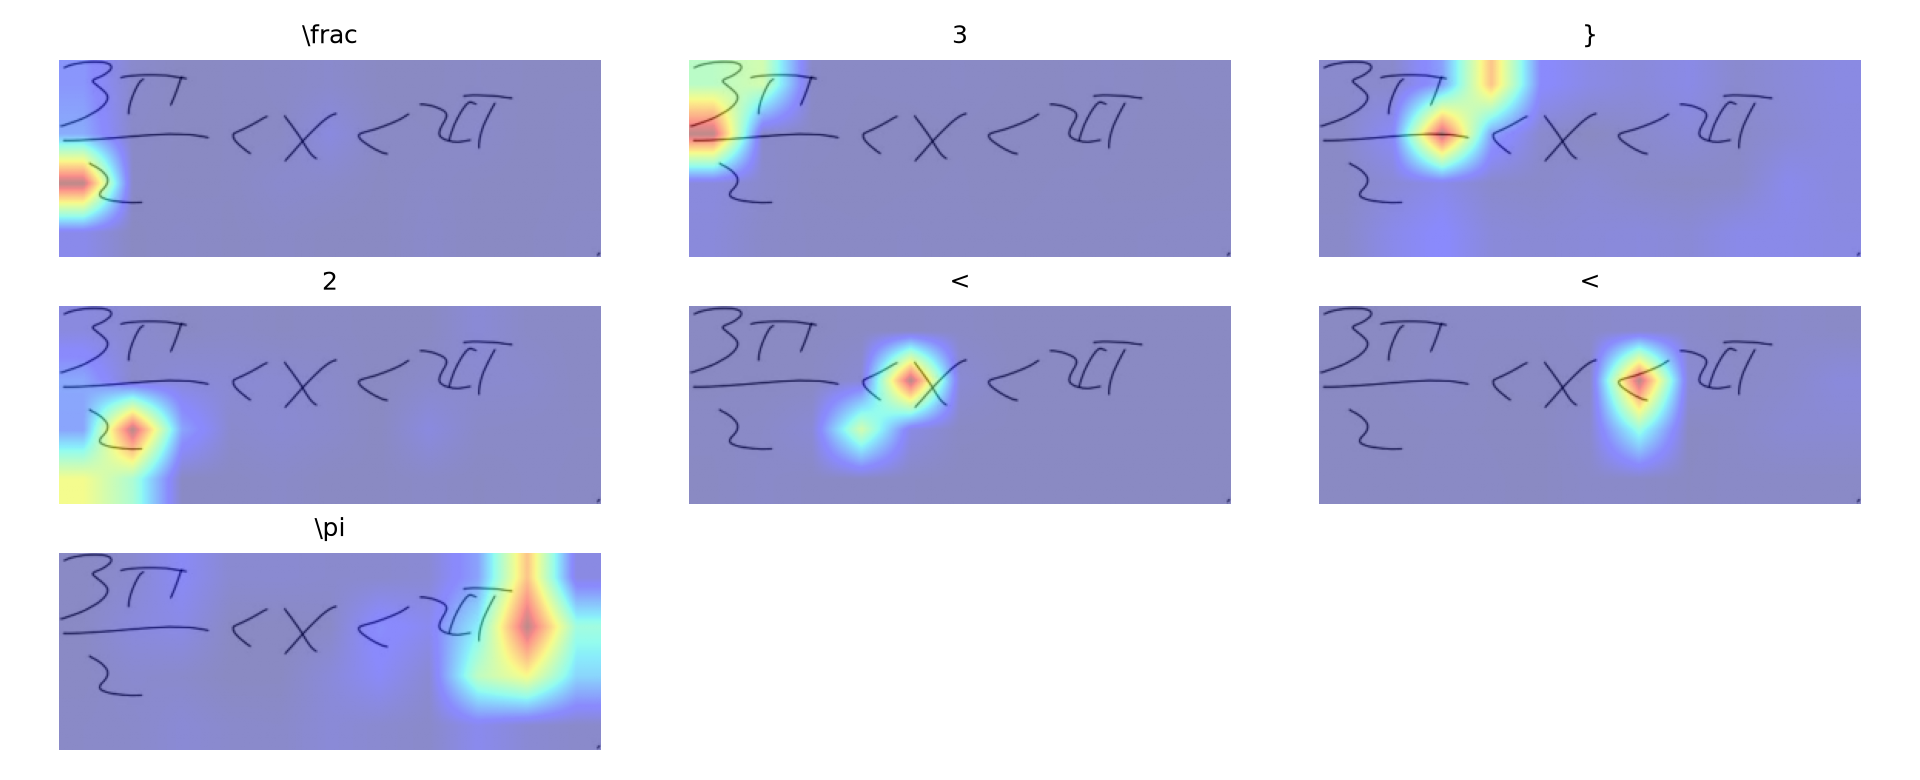
\includegraphics[width=\columnwidth]{figs/att_0000078.png}\\[2pt]
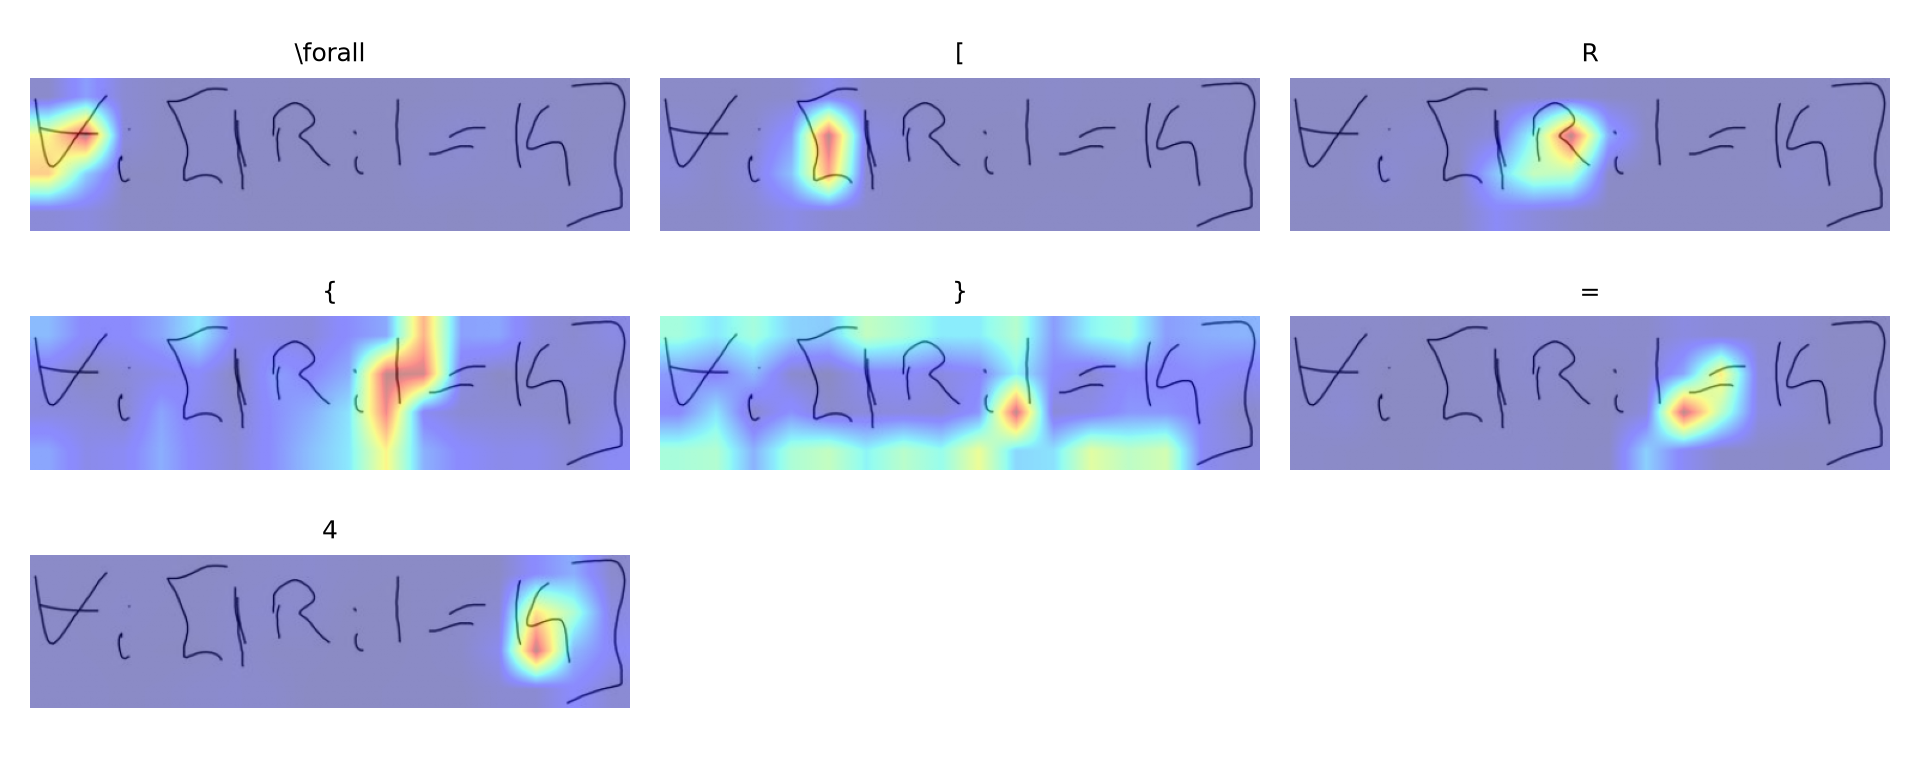
\includegraphics[width=\columnwidth]{figs/att_0000004.png}
\caption{Attention maps of the full-data model for selected decoding steps (panel title = emitted token). Top: correct, $\frac{3\pi}{2}<x<2\pi$. Bottom: incorrect, $\forall i[|R_i|=K]$ read with K as ``14''.}
\label{fig:att}
\end{figure}

\textbf{Confidence.} Because the model outputs a length-normalized probability, uncertain predictions can be flagged to the user. Table~\ref{tab:selective} reports ExpRate when only the most confident fraction of predictions is kept. Accuracy rises steadily as coverage falls, so the confidence score ranks predictions usefully, even though mean confidence on wrong answers (0.880 for the 40k model, 0.927 for the full-data model) is only moderately below that on correct answers (0.953 and 0.976).

\begin{table}[t]
\caption{Selective ExpRate on 500 MathWriting test images: accuracy on the most confident fraction of predictions.}
\label{tab:selective}
\centering
\begin{tabular}{lrrrrr}
\toprule
Model & 100\% & 80\% & 60\% & 40\% & 20\% \\
\midrule
MathWriting 40k & 0.316 & 0.388 & 0.453 & 0.555 & 0.700 \\
MathWriting full & 0.478 & 0.568 & 0.680 & 0.785 & 0.870 \\
\bottomrule
\end{tabular}
\end{table}

\subsection{Limitations}
\begin{itemize}
\item Results in Table~\ref{tab:stages} are on 500-image subsets, not full test splits.
\item The HME100K test set is a slice we carved from the training labels, not the official test set, so it is in-distribution and not comparable with published results.
\item pix2tex is evaluated without fine-tuning on handwriting; a transformer trained under our exact data and budget was not part of this study.
\item The checkpoint is selected by validation cross-entropy, not by ExpRate.
\item We do not evaluate on the CROHME benchmarks, the most widely reported handwritten-expression test sets.
\item Sequential fine-tuning causes forgetting of earlier domains (Section~\ref{sec:results}).
\end{itemize}

%=====================================================================
\section{Conclusion}
A classic ResNet-18 + attention + LSTM model, trained in stages from printed to handwritten to photographed input with a single shared vocabulary, reaches BLEU 79.4 and ExpRate 0.32 on held-out handwritten expressions. Training on the full MathWriting human split raises this to BLEU 86.7 and ExpRate 0.478, while off-the-shelf pix2tex, a printed-formula transformer, recognizes none of the same handwritten expressions exactly. \tbd{one sentence on the ablation} Future work includes evaluation on full and official test splits including CROHME, joint (rather than sequential) multi-domain training to avoid forgetting, and a preprocessing front end (cropping and binarization) for raw phone photographs.

\section*{Acknowledgment}
\tbd{acknowledgment, e.g.\ lab, supervisor, compute (Kaggle)}

%=====================================================================
\begin{thebibliography}{99}
\bibitem{deng2017im2markup} Y.~Deng, A.~Kanervisto, J.~Ling, and A.~M.~Rush, ``Image-to-markup generation with coarse-to-fine attention,'' in \emph{Proc. ICML}, PMLR vol.~70, 2017, pp.~980--989.
\bibitem{zhang2017wap} J.~Zhang, J.~Du, S.~Zhang, D.~Liu, Y.~Hu, J.~Hu, S.~Wei, and L.~Dai, ``Watch, attend and parse: An end-to-end neural network based approach to handwritten mathematical expression recognition,'' \emph{Pattern Recognition}, vol.~71, pp.~196--206, 2017.
\bibitem{bahdanau2015} D.~Bahdanau, K.~Cho, and Y.~Bengio, ``Neural machine translation by jointly learning to align and translate,'' in \emph{Proc. ICLR}, 2015.
\bibitem{xu2015show} K.~Xu \emph{et al.}, ``Show, attend and tell: Neural image caption generation with visual attention,'' in \emph{Proc. ICML}, PMLR vol.~37, 2015, pp.~2048--2057.
\bibitem{tu2016coverage} Z.~Tu, Z.~Lu, Y.~Liu, X.~Liu, and H.~Li, ``Modeling coverage for neural machine translation,'' in \emph{Proc. ACL}, 2016, pp.~76--85.
\bibitem{he2016resnet} K.~He, X.~Zhang, S.~Ren, and J.~Sun, ``Deep residual learning for image recognition,'' in \emph{Proc. CVPR}, 2016, pp.~770--778.
\bibitem{pix2tex} L.~Blecher, ``pix2tex: Using a ViT to convert images of equations into LaTeX code,'' GitHub repository. [Online]. Available: \url{https://github.com/lukas-blecher/LaTeX-OCR}
\bibitem{mathwriting} P.~Gervais, A.~Fadeeva, and A.~Maksai, ``MathWriting: A dataset for handwritten mathematical expression recognition,'' arXiv:2404.10690, 2024.
\bibitem{hme100k} Y.~Yuan \emph{et al.}, ``Syntax-aware network for handwritten mathematical expression recognition,'' in \emph{Proc. CVPR}, 2022, pp.~4553--4562.
\bibitem{papineni2002bleu} K.~Papineni, S.~Roukos, T.~Ward, and W.-J.~Zhu, ``BLEU: a method for automatic evaluation of machine translation,'' in \emph{Proc. ACL}, 2002, pp.~311--318.
\end{thebibliography}

\end{document}
